
\section{Description}\label{description}


\subsection{Navigationsnetz}\label{navigationsnetz}


\subsubsection{Grunds"atzliches}\label{navi_netz_grundsaetzliches}

In der Navigationliste wird zun"achst das logische Netz des Moduls abgebildet,
dar"uber der ``Kurspfad'', der rote zeitlich orientierte Faden durch den
gew"ahlten bzw. durch in Abh"angigkeit vom Benutzerprofil empfohlenen Kurs.\\
Die abgebildete Pfadstruktur ist bewu"st \emph{nicht linear}: Der Studierende
soll neben den reinen Inhalten auch deren Zusammenh"ange und Abh"angigkeit
visuell erleben k"onnen.


\subsubsection{Design der (Sub-)Elemente}\label{}

Die Elemente sollen zun"achst durch farbige, leicht dreidimensional
angedeutete anklickbare K"astchen dargestellt werden (Vorschlag f"ur
1. Entwurf), in denen sich eine Abk"urzung und/oder ein Icon befindet,
das die Art des Elements angibt: T f"ur Theorem, D f"ur Definition,...
(serifenloser Font).\\
Die Subelemente werden in kleineren K"astchen leicht hinter die Elemente
geh"angt, in einheitlicher Farbe und aus Platzgr"unden \textit{ohne} weitere
Unterscheidungsmarkierung. Dabei gelten die Anordnungsregeln aus
Kap. \ref{anordnungsregeln}.\\

Die verf"ugbaren Elemente:
\begin{center}
\begin{tabular}{|l|l|l|}
\hline
Motivation              & (M)   & eigene Farbe          \\
\hline
\hline
Definition              & (D)   & eigene Farbe          \\
\hline
Theorem                 & (T)   & eigene Farbe          \\
\hline
Lemma (Hilfssatz)       & (L)   & Farbe wie Theorem     \\
\hline
Algorithmus             & (Al)  & eigene Farbe          \\
\hline
\hline
Anwendung               & (A)   & eigene Farbe          \\
\hline
\end{tabular}
\end{center}

Die verf"ugbaren Subelemente:
\begin{center}
\begin{tabular}{|l|l|l|l|}
\hline
Herleitung                                      & Her.  & onecolor (grau?)      & oben links\\
\hline
Beweis                                          & Bew.  & onecolor (grau?)      & oben rechts\\
\hline
Bemerkung                                       & Bem.  & onecolor (grau?)      & unten links\\
\hline
Historisches                                    & Hist. & onecolor (grau?)      & unten links\\
\hline
Motivation \footnotesize{(zum Hauptelement)}    & Mot.  & onecolor (grau?)      & unten links\\
\hline
Visualisierung                                  & Vis.  & onecolor (grau?)      & unten rechts\\
\hline
Beispiel                                        & Bsp.  & onecolor (grau?)      & unten rechts\\
\hline
Tabelle                                         & Tab.  & onecolor (grau?)      & unten rechts\\
\hline
\end{tabular}
\end{center}

\clearpage


\subsubsection{An- und Zuordnungsregel der (Sub-)Elemente}\label{anordnungsregeln}

Es gelten die folgenden Anordnungs- und Positionierungsregeln f"ur das
Anh"angen der Subelemente an ihre Elemente (liegen zu einen Element
nicht alle prinzipiell verf"ugbaren Subelemente vor, so r"ucken die
"au"seren nach innen nach):


\begin{enumerate}
\item \textbf{Motivation (zum Modul)}\\
verf"ugb. Subelemente: Historisches, Bem. \hfill{(unten links)}\\
\phantom{verf"ugb. Subelemente: }Visualisierung, Bsp. \hfill{(unten rechts)}\\[-5mm]
\begin{center}
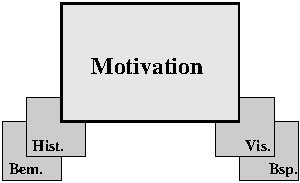
\epsfig{file=Skizzen/elemente_an_mot.eps}
\end{center}
\item \textbf{Definition}\\
verf"ugb. Subelemente: Mot. zu Def., Historisches, Bem. \hfill{(unten links)}\\
\phantom{verf"ugb. Subelemente: }Visualisierung, Bsp., Tabelle \hfill{(unten rechts)}\\[-5mm]
\begin{center}
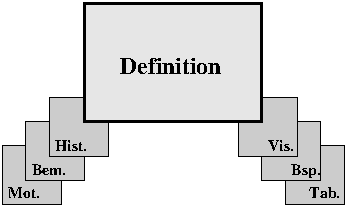
\epsfig{file=Skizzen/elemente_an_def.eps}
\end{center}
\item \textbf{Theorem}\\
verf"ugb. Subelemente: Herleitung \hfill{(oben links)}\\
\phantom{verf"ugb. Subelemente: }Beweis \hfill{(oben rechts)}\\
\phantom{verf"ugb. Subelemente: }Mot. zu Theorem, Historisches, Bem. \hfill{(unten links)}\\
\phantom{verf"ugb. Subelemente: }Visualisierung, Bsp., Tabelle \hfill{(unten rechts)}\\[-5mm]
\begin{center}
\epsfig{file=Skizzen/elemente_an_theorem.eps}
\end{center}

\clearpage

\item \textbf{Lemma}\\
verf"ugb. Subelemente: Herleitung \hfill{(oben links)}\\
\phantom{verf"ugb. Subelemente: }Beweis \hfill{(oben rechts)}\\
\phantom{verf"ugb. Subelemente: }Mot. zu Theorem, Historisches, Bem. \hfill{(unten links)}\\
\phantom{verf"ugb. Subelemente: }Visualisierung, Bsp., Tabelle \hfill{(unten rechts)}\\[-5mm]
\begin{center}
\epsfig{file=Skizzen/elemente_an_lemma.eps}
\end{center}
\item \textbf{Algorithmus}\\
verf"ugb. Subelemente: Mot. zu Algo., Historisches, Bem. \hfill{(unten links)}\\
\phantom{verf"ugb. Subelemente: }Visualisierung, Bsp., Tabelle \hfill{(unten rechts)}\\[-5mm]
\begin{center}
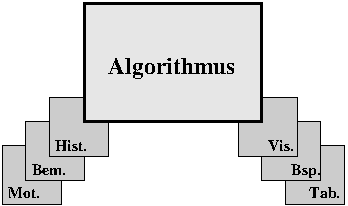
\epsfig{file=Skizzen/elemente_an_algo.eps}
\end{center}
\item \textbf{Anwendung}\\
verf"ugb. Subelemente: Mot. zu Anw., Bem., Historisches \hfill{(unten links)}\\
\phantom{verf"ugb. Subelemente: }Visualisierung, Bsp., Tabelle \hfill{(unten rechts)}\\[-5mm]
\begin{center}
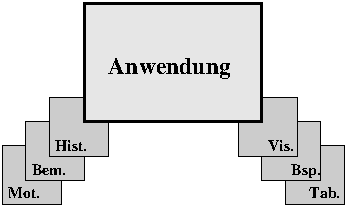
\epsfig{file=Skizzen/elemente_an_anwend.eps}
\end{center}
\end{enumerate}                              


\clearpage

\fbox{\begin{minipage}[t][61mm]{66mm}
\textbf{Motivation:}
\begin{center}
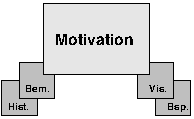
\epsfig{file=Skizzen/elemente_an_mot_mini.eps}
\end{center}
\vfill
verf"ugb. Subelemente:\\[-4ex]
\begin{flushright}
Bem., Historisches\\
Visualisierung, Bsp.
\end{flushright}
\end{minipage}}
\hfill
\fbox{\begin{minipage}[t][61mm]{66mm}
\textbf{Definition:}
\begin{center}
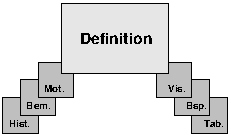
\epsfig{file=Skizzen/elemente_an_def_mini.eps}
\end{center}
\vfill
verf"ugb. Subelemente:\\[-4ex]
\begin{flushright}
Mot. zu ..., Bem., Historisches\\
Visualisierung, Bsp., Tabelle
\end{flushright}
\end{minipage}}

\vspace{3mm}

\fbox{\begin{minipage}[t][61mm]{66mm}
\textbf{Theorem:}
\begin{center}
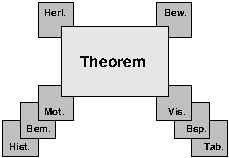
\epsfig{file=Skizzen/elemente_an_theorem_mini.eps}
\end{center}
\vfill
verf"ugb. Subelemente:\\[-4ex]
\begin{flushright}
Herleitung\\
Beweis\\
Mot. zu ..., Bem., Historisches\\
Visualisierung, Bsp., Tabelle
\end{flushright}
\end{minipage}}
\hfill
\fbox{\begin{minipage}[t][61mm]{66mm}
\textbf{Lemma:}
\begin{center}
\epsfig{file=Skizzen/elemente_an_lemma_mini.eps}
\end{center}
\vfill
verf"ugb. Subelemente:\\[-4ex]
\begin{flushright}
Herleitung\\
Beweis\\
Mot. zu ..., Bem., Historisches\\
Visualisierung, Bsp., Tabelle
\end{flushright}
\end{minipage}}

\vspace{3mm}

\fbox{\begin{minipage}[t][61mm]{66mm}
\textbf{Algorithmus:}
\begin{center}
\epsfig{file=Skizzen/elemente_an_algo_mini.eps}
\end{center}
\vfill
verf"ugb. Subelemente:\\[-4ex]
\begin{flushright}
Mot. zu ..., Bem., Historisches\\
Visualisierung, Bsp., Tabelle
\end{flushright}
\end{minipage}}
\hfill
\fbox{\begin{minipage}[t][61mm]{66mm}
\textbf{Anwendung:}
\begin{center}
\epsfig{file=Skizzen/elemente_an_anwend_mini.eps}
\end{center}
\vfill
verf"ugb. Subelemente:\\[-4ex]
\begin{flushright}
Mot. zu ..., Bem., Historisches\\
Visualisierung, Bsp., Tabelle
\end{flushright}
\end{minipage}}

\clearpage

\subsubsection{Verbindungslinien}\label{}

Es existieren zwei Arten von Verbindungslinien: 

\begin{list_sabina}
        \item \textbf{logisches Netz}
        \item \textbf{Kurspfad} 
\end{list_sabina}


\paragraph{Das logische Netz}\mbox{ }\\[-2ex]

Die logischen Abh"angigkeiten werden durch (d"unne, schwarze?) Linien
zwischen den Elementen abgebildet, soweit sie im
mathematisch-fachlichen Sinn bestehen.

Das bedeutet insbesondere: \\
Motivationen werden stets an erster Position gezeichnet, aber nicht
durch Linien mit dem Anschlu"selement verbunden.\\
Anwendungen werden in letzter Position gezeichnet und ebenfalls nicht
verbunden.\\
Definitionen, Theoreme, Lemmata und Algorithmen bilden zentralen
mittleren Block und m"ussen stets untereinander verbunden werden. An
jeder Gabelung wird zwischen ``und''- und ``oder''-Verbindung
unterschieden (``+''-Icon f"ur und, ``oder'' ohne Icon).

\begin{figure}[h]
\begin{center}
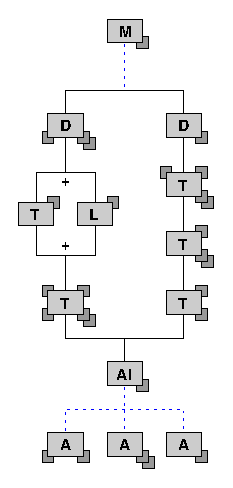
\epsfig{file=Skizzen/navi_drittel.eps}
\caption{Logischer Pfad, logische Verbindungen, ohne Kurspfad}
\end{center}
\end{figure}

\clearpage

\paragraph{Der Kurspfad}\mbox{ }\\[-2ex]

"Uber das Netz der logischen Abh"angigkeiten wird ein ``roter Faden''
gelegt, der der linearen Anordnung der Inhalte in einem Kurs
entspricht.

Das bedeutet insbesondere: \\
``Oder''-Verzweigungen f"uhren auf i.f. unterschiedliche Kurse; f"ur
jede auftretende ``Oder''-Verzweigung mu"s daher ein eigenes Bild
generiert werden.\\
Bei ``Und''-Verbindungen m"ussen (in einer definierten Reihenfolge) beide
Teile durchlaufen werden, der rote Faden liegt daher nicht mehr auf
den logischen Linien (siehe Abb. \ref{kurs_mit_rotem_faden}).

\begin{figure}[h]
\begin{center}
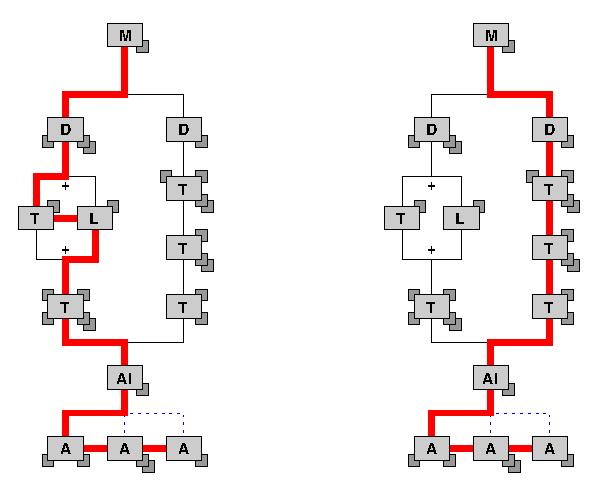
\epsfig{file=Skizzen/navi_drittel_kurs.eps}
\caption{M"ogliche Kurspfade mit rotem Faden}\label{kurs_mit_rotem_faden}
\end{center}
\end{figure}

Um den aktiven Kurspfad zus"atzlich hervorzuheben, sollte der nicht
zum Kurspfad geh"orende Teil leicht in den Hintergrund gelegt werden,
ohne aber seine Funktionalit"at grunds"atlich zu verlieren.







\subsubsection{Verbindungslinien}\label{}


Der ``Forward/Backward-Button'' erm"oglicht die Bewegung entlang des
roten Fadens in einfacher Weise, 
auch k"onnen die K"astchen alternativ \textit{direkt} angeklickt werden
(damit stehen dem Benutzer immer auch andere Reihenfolge zur 
Verf"ugung).

Die Art des Elemente und Subelemente mu"s durch Farben, Icons oder
"ahnliches gekennzeichnet sein\footnote{F"ur Beschriftung sind
mindestens die Subelemente viel zu klein, die Elemente k"onnten
\textit{einen} Buchstaben tragen; diese Gr"o"senbeschr"ankung
entsteht, weil einerseits das Navigationsnetz keinesfalls durch
Scrollbars zerst"uckelt werden darf, andererseits aber ein gesamtes
Modul darstellen soll.}.


\subsubsection{Zus"atzliche Effekte}\label{navi_netz_zusaetzliche_effekte}

Mouse-Aktionen k"onnen weitere "Ubersichtsm"oglichkeiten schaffen:

\begin{list_sabina}
        \item \textbf{Mouse-over}\\
        Zoom-Effekt, Element mit seinen Subelementen erscheint
        vergr"o"sert und mit Mini-Abstrakt/Titel
        \item \textbf{Mouse-out}\\
        Zoom-Effekt verschwindet wieder
        \item \textbf{Left-Mouse-Click}\\
        Inhalt erscheint im zentralen Inhaltsfenster
        \item \textbf{Right-Mouse-Click}\\
        Inhalt erscheint, aber in Extrafenster (zum ``Festhalten'')
\end{list_sabina}


\subsection{Lineare Navigation}\label{Lineare Navigation}






